\chapter{Anexo I - Pliego de condiciones}

Este anexo se ha añadido siguiendo la recomendación oficial de la \gls{uah} sobre \gls{tfg}s. En él se indicarán las condiciones materiales de las distintas máquinas donde se ha desarrollado el proyecto. Por último, se resumirán tanto las limitaciones de \textit{hardware}, como las especificaciones del \textit{software} instalado en las máquinas virtuales donde se llevó a cabo los distintos casos de uso. 

\section{Condiciones materiales y equipos}

A continuación, se muestran todos los materiales que se han utilizado en el proyecto. Únicamente se indicarán las características de los materiales vitales para el desarrollo del \gls{tfg}. De este modo, se pretende que queden recogidos todas las especificaciones técnicas con las se han realizado las pruebas y validaciones del desarrollo.

\subsection{Especificaciones Máquina A}
\label{maquina_A}
    \begin{itemize}
        \item Procesador: Intel(R) Core(TM) i7-4790 CPU @ 3.60Ghz
        \item Memoria: 16GB DRR4 (2 slots de 8GB)
        \item Gráfica: GeForce GTX 970 Windforce - 4GB
        \item Sistema operativo: Windows 10 - v1909 (Compilación 18363.836)
    \end{itemize}
    
\subsection{Especificaciones Máquina B}
\label{maquina_B}
    \begin{itemize}
        \item Procesador: Intel Core i7-8750H, Hexa Core 2.2GHz-4.1GHz
        \item Memoria: 16GB DDR4, 2400MHz
        \item Gráfica: GeForce GTX0150Ti-4GB GDDR5
        \item Sistema operativo: Windows 10 - v1903 (Compilación 18362.836)
    \end{itemize}


\subsection{Especificaciones máquinas virtuales}
Todas las máquinas virtuales se han ejecutado sobre la máquina B (\ref{maquina_B}), y se ha conectado a ellas vía SSH con la máquina A (\ref{maquina_A}). Las máquinas virtuales se desplegaron sobre el hipervisor \textbf{VirtualBox}\footnote{\url{https://www.virtualbox.org/}}, haciendo uso de su versión \texttt{v6.0.14 r133895 (Qt5.6.2)}. Dado que había dos entornos de desarrollo muy definidos, como son el entorno P4 y el entorno \gls{xdp}, se crearon dos máquinas virtuales pudiendo así aislar posibles conflictos de dependencias. Las dependencias de cada máquina virtual para poder replicar los casos de uso, se pueden instalar haciendo uso de los scripts de instalación suministrados en el repositorio del \gls{tfg}\footnote{https://github.com/davidcawork/TFG}, pudiendo cualquier interesado replicar los escenarios sin mayor complicación. \\

\par

\subsubsection{Máquina virtual entorno P4}
\vspace{0.5cm}
\label{maquina_p4}
    \begin{itemize}
        \item Procesador: Intel Core i7-8750H, 2 cores 2.2GHz-4.1GHz
        \item Memoria: 8GB DDR4, 2400MHz
        \item Sistema operativo: Ubuntu 16.04.6 LTS x86\_64
        \item Kernel: \texttt{4.15.0-88-generic}
        \item Configuración de red: Modo bridge, conectado a interfaz Intel(R) Wireless-AC 9560
    \end{itemize}
    \vspace{1cm}
    \begin{figure}[ht]
        \centering
        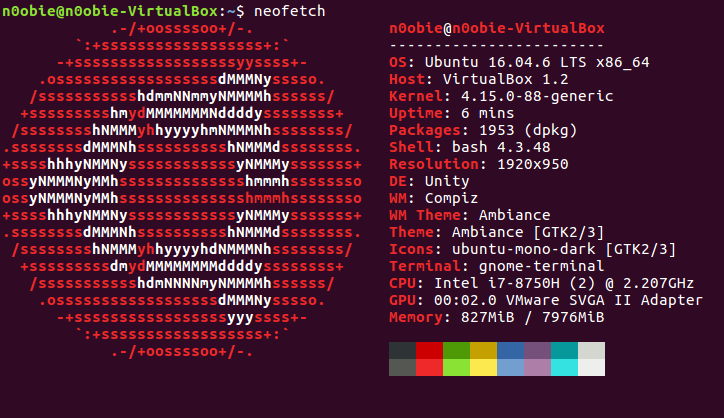
\includegraphics[width=12cm]{archivos/img/anexos/VM_p4_edited.png}
        \caption{Especificaciones de la máquina virtual P4}
        \label{fig:VM_p4}
    \end{figure}
\newpage    
\subsubsection{Máquina virtual entorno XDP}
\label{maquina_xdp}
\vspace{0.5cm}
    \begin{itemize}
        \item Procesador: Intel Core i7-8750H, 6 cores 2.2GHz-4.1GHz
        \item Memoria: 4GB DDR4, 2400MHz
        \item Sistema operativo: Ubuntu 18.04.3 LTS x86\_64
        \item Kernel: \texttt{5.3.0-40-generic}
        \item Configuración de red: Modo bridge, conectado a interfaz Intel(R) Wireless-AC 9560
    \end{itemize}
    \vspace{1cm}
        \begin{figure}[ht]
        \centering
        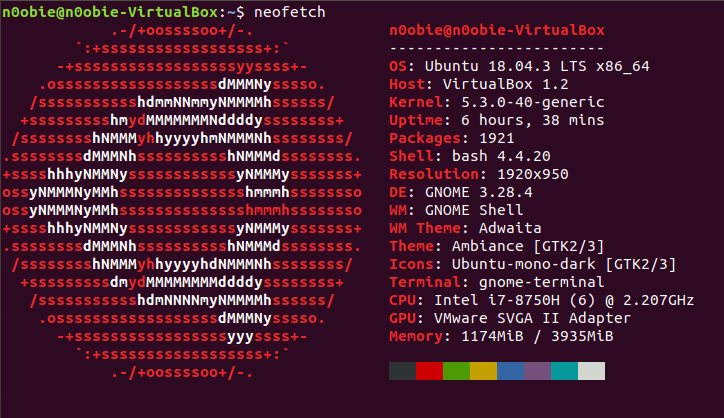
\includegraphics[width=12cm]{archivos/img/anexos/VM_xdp_edited.png}
        \caption{Especificaciones de la máquina virtual XDP}
        \label{fig:VM_xdp}
    \end{figure}


